\documentclass[14pt, a0paper, landscape, margin=0mm, innermargin=15mm,
   blockverticalspace=15mm, colspace=15mm, subcolspace=8mm]{tikzposter}
\usepackage[T1]{fontenc}
\usepackage{amssymb}
\usepackage{float}
\usepackage{amsmath}
\usepackage{caption}
\usepackage{color}
\usepackage[backend=bibtex]{biblatex}
\addbibresource{references.bib}
\setlength{\tabcolsep}{2em}

% title, author, and institution
\title{\fontsize{99pt}{1em}\selectfont\hspace{-3em} A Positivity-preserving Scheme for Radiation Transport}
\author{\begin{tabular}{c c c}
  Jean C. Ragusa       & Jean-Luc Guermond      & Joshua E. Hansel\\
  jean.ragusa@tamu.edu & guermond@math.tamu.edu & joshhansel@tamu.edu\\
  Texas A\&M University & Texas A\&M University & Texas A\&M University
\end{tabular}}

% custom background style
\definebackgroundstyle{mybackground}{
  \node[at=(current page.center)] at (0,0) {
\includegraphics[height=\textheight]{figures/blue_gradient.png}};
}

% custom block style
\defineblockstyle{myblockstyle}{
  titlewidthscale=1.0, bodywidthscale=1, titlecenter,
  titleoffsetx=0pt, titleoffsety=0pt, bodyoffsetx=0mm, bodyoffsety=15mm,
  bodyverticalshift=10mm, roundedcorners=0, linewidth=0pt,
  titleinnersep=6mm, bodyinnersep=1cm
}{
  \draw[color=framecolor, fill=blockbodybgcolor,
  rounded corners=\blockroundedcorners, line width=\blocklinewidth] (blockbody.south west)
  rectangle (blockbody.north east);
  \ifBlockHasTitle
    \draw[color=framecolor, fill=blocktitlebgcolor,
    rounded corners=\blockroundedcorners, line width=\blocklinewidth] (blocktitle.south west)
    rectangle (blocktitle.north east);
  \fi
}

% custom color style
\definecolorstyle{mycolorstyle} {
  \definecolor{colorOne}{named}{green}
  \colorlet{colorTwo}{black!45!white!45!blue}
  \colorlet{colorThree}{red}
}{
  % Background Colors
  \colorlet{backgroundcolor}{colorOne}
  \colorlet{framecolor}{colorTwo}
  % Title Colors
  \colorlet{titlefgcolor}{white}
  \colorlet{titlebgcolor}{colorOne}
  % Block Colors
  \colorlet{blocktitlebgcolor}{colorTwo}
  \colorlet{blocktitlefgcolor}{white}
  \colorlet{blockbodybgcolor}{white}
  \colorlet{blockbodyfgcolor}{black}
  % Innerblock Colors
  \colorlet{innerblocktitlebgcolor}{white}
  \colorlet{innerblocktitlefgcolor}{black}
  \colorlet{innerblockbodybgcolor}{colorThree!30!white}
  \colorlet{innerblockbodyfgcolor}{black}
  % Note colors
  \colorlet{notefgcolor}{black}
  \colorlet{notebgcolor}{colorTwo!50!white}
  \colorlet{noteframecolor}{colorTwo}
}

% theme and style and colors
\usetheme{Autumn} % Default, Rays, Basic, Simple, Envelope, Wave, Board, Autumn, and Desert
\usebackgroundstyle{mybackground} % Default, Rays, VerticalGradation, BottomVerticalGradation, Empty
\usecolorstyle{mycolorstyle} % Default, Australia, Britain, Sweden, Spain, Russia, Denmark, Germany
\usetitlestyle{Empty} % Default, Basic, Envelope, Wave, VerticalShading, Filled, Empty
\useblockstyle{myblockstyle} % Default, Basic, Minimal, Envelope, Corner, Slide, TornOut

\newcommand{\tcr}[1]{\textcolor{black}{#1}}

% document
%--------------------------------------------------------------------------------
\begin{document}\maketitle
\begin{columns}

% FIRST COLUMN
\column{0.25}
  \block{\centering INTRODUCTION}{
    \setlength{\parskip}{0.5\baselineskip}
    \vspace{-\parskip}
    The transport equation, also called the Boltzmann equation, describes the
transport of particles or waves through some background media and some
of its applications include nuclear reactors, atmospheric science, radiation
therapy, astrophysics, radiation shielding, and high energy density physics.
In this paper, focus is on solution techniques applicable to the first-order
form of the transport equation, discretized in angle with discrete ordinates,
which gives what is commonly called the $S_N$ equations:
\begin{equation}\label{eq:transport_scalar}
  \frac{1}{v(E)}\ppt{\aflux} + \di\cdot\nabla\aflux\xdet
    + \totalxsec\xet\aflux\xdet = \Qtot\xdet
  \eqc
\end{equation}
where $\Qtot\xdet$ denotes the sum of the extraneous source, prompt and delayed
fission sources, and scattering source:
\begin{multline}
  \Qtot\xdet \equiv \Qext\xdet\\
    + \frac{\chi_\text{p}(E)}{4\pi}\int\limits_0^\infty
      dE'\nu_\text{p}(\x,E',t)\fissionxsec(\x,E',t)\phi(\x,\di,E',t)
    + \sum\limits_{i=1}^{n_\text{d}}\frac{\chi_{\text{d},i}(E)}{4\pi}\lambda_i C_i\xt\\
    + \int\limits_0^\infty dE'\int\limits_{4\pi}d\di'
      \scatteringxsec(\x,E'\rightarrow E,\di'\rightarrow\di,t)\aflux(\x,\di',E',t)
  \eqp
\end{multline}
The $S_N$ equations are an attractive form of the transport equation because
the $S_N$ equations can be decoupled by using iterative techniques for the
scattering source, an approach called source iteration \cite{glasstone}:
\begin{equation}
  \frac{1}{v}\ppt{\aflux^{(\ell)}}
    + \di\cdot\nabla\aflux^{(\ell)}
    + \totalxsec\aflux^{(\ell)} = \Qtot^{(\ell-1)} \eqc
\end{equation}
where $\ell$ is the iteration index. The decoupling of the equations allows
scalar solution techniques to be leveraged.
Traditionally, the preferred spatial discretization method for the $S_N$
equations is the Discontinuous Galerkin finite element method (DGFEM)
\cite{Lesaint1974}\cite{Reed_Hill_1973}. Here, however, the
Continuous Galerkin finite element method (CGFEM) is applied. There
has been some recent work by Guermond and Popov \cite{guermond_ev} on
solution techniques for conservation laws with CGFEM, which addresses some
of the main disadvantages of CGFEM versus DGFEM, including the formation
of spurious oscillations. This work aims to demonstrate a proof of concept
for the application of these solution techniques to the transport equation.
Furthermore, some or all of the methodology explored in this paper may be
later extended to DGFEM as well \cite{zingan_2013}.

One of the main objectives of this paper is to present a method that precludes
the formation of spurious oscillations and the negativities that result from
these oscillations. The occurrence of negativities in the numerical solution of
the transport equation has been a long-standing issue \cite{lanthrop}.
Not only are these negativities physically inaccurate, but they can cause
simulations to terminate prematurely. Many attempts to remedy this
issue rely on ad-hoc fix-ups, such as the set-to-zero fix-up for the
classic diamond difference scheme \cite{lewis}. Recent work by Hamilton
introduced a similar fix-up for the linear discontinuous finite element
method (LDFEM) that conserves local balance and preserves third-order accuracy.
Walters and Wareing developed characteristic methods \cite{walters_NC}, but
Wareing later notes that these characteristic methods are difficult to
implement and offers a nonlinear positive spatial differencing scheme
known as the exponential discontinuous scheme \cite{wareing}.
Maginot has recently developed a consistent set-to-zero (CSZ) LDFEM
method \cite{maginot}, as well as a non-negative method for bilinear
discontinuous FEM \cite{maginot_mc2015}.

Traditional approaches to remedy the spurious oscillation issue included
the flux-corrected transport (FCT) algorithm, introduced in 1973 for finite
difference discretizations
by Boris and Book \cite{borisbook}, which has since been applied to the finite
element method \cite{kuzmin_FCT}. The idea of FCT is to blend a low-order scheme
having desirable properties with a scheme of a higher order of accuracy.

Recent work by Guermond and Popov addresses the issue of spurious oscillations
for general conservation laws by using artificial dissipation based on
local entropy production, a method known as entropy viscosity \cite{guermond_ev}.
The idea of entropy viscosity is to enforce an entropy inequality on the weak solution,
and thus filter out weak solutions containing spurious oscillations. However,
entropy viscosity solutions may still contain spurious
oscillations, albeit smaller in magnitude, and consequently negativities
are not precluded. To circumvent this deficiency, Guermond proposed using
the entropy viscosity method in conjunction with the FCT
algorithm \cite{guermond_secondorder}; the high-order scheme component in FCT,
traditionally the unmodified Galerkin scheme, is replaced with the entropy
viscosity scheme.
For the low-order
scheme, Guermond also introduced
a discrete maximum principle (DMP) preserving (and positivity-preserving)
scheme for scalar
conservation laws \cite{guermond_firstorder}.

This paper presents an FCT scheme that is largely rooted in the work by Guermond
and Popov, but is extended to allow application to the transport equation,
which does not fit the prototype of a conservation law but is instead a
balance law, which includes sinks and sources, namely the reaction term
$\totalxsec\aflux$ and the source term $\Qtot$. The presence
of these terms is also a novelty in the context of the FCT algorithm.
In addition, much of the present work on FCT has been for fully explicit time
discretizations, although there has been some work on implicit time discretizations
as well. Because speeds in radiation transport (such as the speed of light)
are so large, implicit and steady-state time discretization are important
considerations, given the CFL time step size restriction for fully explicit
methods. Thus this paper also considers implicit and steady-state FCT, which
has been implemented before \cite{implicit_FCT}.

This paper is organized as follows. Section \ref{sec:preliminaries} gives
some preliminaries such as the problem formulation and discretization.
Recall that the FCT algorithm uses a low-order scheme and a high-order scheme.
Section \ref{sec:low} presents the low-order scheme, Section \ref{sec:high}
presents the high-order scheme (which is based on entropy viscosity),
and Section \ref{sec:fct} presents the FCT scheme that combines the two. Then, Section
\ref{sec:results} presents results for a number of test problems, and
Section \ref{sec:conclusions} gives conclusions.

  }
  \block{\centering CFEM DISCRETIZATION}{
    \setlength{\parskip}{0.5\baselineskip}
    \vspace{-\parskip}
    Testing with each FEM basis function $\varphi_i(\mathbf{x})$ gives a linear system:

\begin{equation}\label{eq:semidiscrete}
      \mathbf{M}^C\frac{d\mathbf{U}}{dt}+\mathbf{A} \mathbf{U}(t) = \mathbf{b},
\end{equation}

\begin{equation}
	M^C_{i,j} \equiv \int\limits_{S_{i,j}}
    \varphi_j\varphi_i dV, \qquad
  A_{i,j} = \int\limits_{S_{i,j}}\left(
   \mathbf{v}\cdot\nabla\varphi_j +
   \sigma\varphi_j\right)\varphi_i dV, \qquad
	b_i \equiv \int\limits_{S_i} q\varphi_i dV.
\end{equation}

To discretize Eqn.~\ref{eq:semidiscrete} in time, fully explicit
temporal discretization schemes are used, such as explicit Euler,

\begin{equation}\label{eq:exgalerkin}
   \mathbf{M}^C\frac{\mathbf{U}^{n+1}-\mathbf{U}^n}{\Delta t}
     + \mathbf{A}\mathbf{U}^n = \mathbf{b}^n.
\end{equation}

and 3rd-order SSP (SSP3) explicit methods.

  }
  \block{\centering LOW-ORDER SCHEME}{
    \setlength{\parskip}{0.5\baselineskip}
    \vspace{-\parskip}
    A \underline{\bf monotonicity-preserving, positivity-preserving low-order} scheme
is defined by lumping the mass matrix and adding a low-order diffusion
operator:

\begin{equation}\label{eq:loworderscheme}
   \mathbf{M}^L\frac{\mathbf{U}^{L,n+1}-\mathbf{U}^n}{\Delta t}
      +\left(\mathbf{A}+\tcr{\mathbf{D}^L}\right)\mathbf{U}^n = \mathbf{b},
\end{equation}

where the diffusion matrix $\tcr{\mathbf{D}^L}$ entries are computed using a local low-order
viscosity and viscous bilinear form:

\begin{equation}\label{eq:loworderD}
   \tcr{D^L_{i,j}} = \sum\limits_{K\subset S_{i,j}}\nu_K^L b_K(\varphi_j,\varphi_i).
\end{equation}

The local viscous bilinear form for an element $K$ takes a graph-theoretic
approach introduced by Guermond~\cite{guermond_firstorder}:

\begin{equation}\label{eq:bilinearform}
      b_K(\varphi_j, \varphi_i) \equiv \left\{\begin{array}{l l}
         -\frac{1}{n_K - 1}V_K & i\ne j, \quad i,j\in \mathcal{I}(K),\\
         V_K                   & i = j,  \quad i,j\in \mathcal{I}(K),\\
         0                     & i\notin\mathcal{I}(K) \quad | \quad j\notin\mathcal{I}(K),
      \end{array}\right.
\end{equation}

where $V_K$ is the volume of cell $K$,
$\mathcal{I}(K)\equiv \{j\in\{1,\ldots,N\}: |S_j\cap K|\ne 0\}$
is the set of indices corresponding to degrees of freedom in
the support of cell $K$, and $n_K \equiv \mbox{card}(\mathcal{I}(K))$.
The local low-order viscosity is defined as the following:

\begin{equation}
   \nu_K^L \equiv \max\limits_{i\ne j\in \mathcal{I}(K)}\frac{\max(0,A_{i,j})}
      {-\sum\limits_{T\subset S_{i,j}} b_T(\varphi_j, \varphi_i)},
\end{equation}

If the CFL condition $\Delta t \leq \frac{M_{i,i}^L}{A_{i,i}^L}$
is satisfied for all $i$, then the explicit
low-order scheme given in Eqn. \ref{eq:loworderscheme} \underline{\bf satisfies the following
discrete maximum principle}:

\begin{equation}\label{eq:dmp}
   U_{\min,i}^n\left(1-\frac{\Delta t}{M_{i,i}^L}
      \sum\limits_j A^L_{i,j}\right)
      + \frac{\Delta t}{M_{i,i}^L}b_i\leq
   U_i^{L,n+1}\leq
   U_{\max,i}^n\left(1-\frac{\Delta t}{M_{i,i}^L}
      \sum\limits_j A^L_{i,j}\right)
      + \frac{\Delta t}{M_{i,i}^L}b_i\quad\forall i,
\end{equation}

where $U_{\min,i}^n = \min\limits_{j\in \mathcal{I}(S_i)}U_j^n$,
$U_{\max,i}^n = \max\limits_{j\in \mathcal{I}(S_i)}U_j^n$
and $\mathcal{I}(S_i)$ is the set of indices of degrees of freedom in the
support of degree of freedom $i$.

  }

% SECOND COLUMN
\column{0.25}
  \block{\centering HIGH-ORDER SCHEME}{
    \setlength{\parskip}{0.5\baselineskip}
    \vspace{-\parskip}
    \begin{subequations}
\begin{equation}
  \diffusionmatrixletter^{\entropy,\timeindex}\ij \equiv
    \nodequantity{\diffusionmatrixletter}^{\entropy,\timeindex}\nodeij \eqc
\end{equation}
\begin{equation}
  \nodequantity{\diffusionmatrixletter}^{\entropy,\timeindex}\kl \equiv
    \frac{\entropyresidualcoef\nodequantity{\entropyresidual}\kl^n +
      \entropyjumpcoef\nodequantity{\entropyjump}\kl^n}
      {\nodequantity{\entropynormalization}^\timeindex\kl}
  \eqc
\end{equation}
\end{subequations}
where
\begin{equation}
  \nodequantity{\entropyresidual}\kl^\timeindex \equiv \left|
    \int\limits_{\nodequantity{\support}\kl}
      \entropyresidual(\vectorsolution^\timeindex,\vectorsolution^{\timeindex-1})
      \nodequantity{\testfunction}_k(\x)
      \nodequantity{\testfunction}_\ell(\x) \dvolume
    \right|
  \eqc
\end{equation}
% TODO: I think the following quantity is always zero because the product
% of the supports on the faces are zero, so the jumps may need
% to be redefined or omitted.
\begin{equation}
  \nodequantity{\entropyjump}\kl^\timeindex \equiv \maxcelldiameter
    \sum\limits_{F:\facedomain_F\subset\nodequantity{\support}\kl} \,
    \int\limits_{\facedomain_F}\entropyjump_F(\vectorsolution^\timeindex)
      \nodequantity{\testfunction}_k(\x)
      \nodequantity{\testfunction}_\ell(\x) \darea
  \eqc
\end{equation}
\begin{equation}
  \nodequantity{\entropynormalization}^\timeindex\kl \equiv
    \max\limits_{\cell:\celldomain\subset\nodequantity{\support}\kl}
    \max\limits_{\qpoint\in\quadraturepoints(\celldomain)}
    \entropynormalization(\vectorsolution^\timeindex(\qpoint))
  \eqp
\end{equation}
Similarly to the scalar case, the high-order diffusion uses the low-order
diffusion as an upper bound:
\begin{subequations}
\begin{equation}
  \diffusionmatrixletter^{\high,\timeindex}\ij \equiv
    \nodequantity{\diffusionmatrixletter}^{\high,\timeindex}\nodeij \eqc
\end{equation}
\begin{equation}
  \nodequantity{\diffusionmatrixletter}^{\high,\timeindex}\kl \equiv
    \min\pr{\nodequantity{\diffusionmatrixletter}^{\entropy,\timeindex}\kl,
      \nodequantity{\diffusionmatrixletter}^{\low,\timeindex}\kl}
  \eqc
\end{equation}
\end{subequations}

  }
  \block{\centering FCT SCHEME}{
    \setlength{\parskip}{0.5\baselineskip}
    \vspace{-\parskip}
    Recall that FCT defines antidiffusive correction fluxes from a low-order,
monotone scheme to a high-order scheme. Calling these fluxes
$\correctionfluxvector$, this gives
\begin{equation}
  \lumpedmassmatrix\frac{\solutionvector^{H,n+1}-\solutionvector^n}{\dt}
    + (\ssmatrix+\diffusionmatrix^L)\solutionvector^n = \ssrhs^n
    + \correctionfluxvector \eqp
\end{equation}
Subtracting the high-order scheme equation from this gives the
definition of $\correctionfluxvector$:
\begin{equation}
  \correctionfluxvector \equiv
    -(\consistentmassmatrix-\lumpedmassmatrix)
    \frac{\solutionvector^{H,n+1}-\solutionvector^n}{\dt}
    + (\diffusionmatrix^L-\diffusionmatrix^{H,n})\solutionvector^n \eqp
\end{equation}
Now it is necessary to decompose these fluxes into internodal fluxes
$\correctionfluxij$ such that $\sum_j\correctionfluxij=\correctionfluxletter_i$:
\begin{equation}
  \correctionfluxij = -M\ij^C\pr{
    \frac{\MakeUppercase{\solutionletter}^{H,n+1}_j
      -\MakeUppercase{\solutionletter}^n_j}{\Delta t}
    -\frac{\MakeUppercase{\solutionletter}^{H,n+1}_i
      -\MakeUppercase{\solutionletter}^n_i}{\Delta t}
  }
  + (D\ij^L-D\ij^{H,n})(\MakeUppercase{\solutionletter}^n_j
    -\MakeUppercase{\solutionletter}^n_i) \eqp
\end{equation}
Recall that the objective of FCT is to limit these antidiffusive
fluxes to enforce some physical bounds. For the scalar case, one can use
the discrete maximum principle bounds given by Equation \eqref{eq:dmp}.
The limitation is achieved by applying a limiting coefficient $L\ij$ to each
internodal flux $\correctionfluxij$:
\begin{equation}
  \lumpedmassmatrix\frac{\solutionvector^{n+1}-\solutionvector^n}{\dt}
    + \ssmatrix^L\solutionvector^n = \ssrhs
    + \limitermatrix\cdot\correctionfluxmatrix \eqp
\end{equation}
Each limiting coefficient is between zero and unity: $0\leq L\ij\leq 1$.
   \begin{itemize}
      \item If all $L\ij$ are zero, then the low-order scheme is produced.
      \item If all $L\ij$ are one, then the high-order scheme is produced.
   \end{itemize}
   \item The enforced bounds can be rearranged to bound the limited flux sums:
      \begin{equation}
         Q^-_i \leq \sum\limits_j L\ij \correctionfluxij \leq Q^+_i \eqc
      \end{equation}
      where $Q_i^\pm$ has the following definition:
      \begin{equation}
         Q_i^\pm \equiv M_{i,i}^L\frac{W_i^\pm-U_i^n}{\Delta t}
         + \sum\limits_j A_{i,j}^L U_j^n - b_i \eqp
      \end{equation}
   \item The classic Zalesak limiting strategy starts by separating the
      negative and positive fluxes:
      \begin{equation}
         Q^-_i \leq \sum\limits_{j:\correctionfluxij<0} L\ij \correctionfluxij +
            \sum\limits_{j:\correctionfluxij>0} L\ij \correctionfluxij\leq Q^+_i \eqp
      \end{equation}
      The positive fluxes risk violating $Q_i^+$, and the negative fluxes risk
      violating $Q_i^-$.
   \item Zalesak's limiting coefficients assume that
      all positive fluxes into a node $i$ have the same limiting coefficient
      $L^+_i$ and similarly, negative fluxes have the same limiting coefficient
      $L^-_i$:
      \begin{equation}
        Q^-_i \leq L^-_i \correctionfluxletter^-_i
          + L^+_i \correctionfluxletter^+_i \leq Q^+_i \eqp
      \end{equation}
      where
      \begin{equation}
        \correctionfluxletter_i^- \equiv \sum\limits_{j:\correctionfluxij<0}
          \correctionfluxij \eqc \qquad
        \correctionfluxletter_i^+ \equiv \sum\limits_{j:\correctionfluxij>0}
          \correctionfluxij \eqp
      \end{equation}
   \item As a conservative bound for $L^+_i$, contributions from negative fluxes
      are ignored (pretending $L_i^-=0$), giving
      $L^+_i \leq \frac{Q_i^+}{\correctionfluxletter_i^+}$
      and similarly for $L^-_i$ and the lower bound.
   \item Then, recalling that limiting coefficients are not greater than unity:
      \begin{equation}
         L_i^\pm \equiv\left\{
            \begin{array}{l l}
               1 & \correctionfluxletter_i^\pm = 0\\
               \min\left(1,\frac{Q_i^\pm}{\correctionfluxletter_i^\pm}\right) &
                 \correctionfluxletter_i^\pm \ne 0
            \end{array}
            \right. \eqp
      \end{equation}
   \item However, to limit fluxes conservatively, limited correction fluxes must
      be equal and opposite:
      \begin{equation}
        L\ij \correctionfluxij = -L_{j,i}
          \MakeUppercase{\correctionfluxletter}_{j,i} \eqp
      \end{equation}
      Since $\correctionfluxij$ happens to be skew symmetric
      ($\MakeUppercase{\correctionfluxletter}_{j,i}=-\correctionfluxij$) due to the
      chosen flux decomposition, the limiting coefficients must be symmetric:
      $L_{j,i} = L\ij$.
   \item Thus when deciding the limiting coefficient $L\ij$ for a flux $\correctionfluxij$, 
      one must not only consider the bounds for $i$ but also the bounds for $j$.
      Specifically, a positive flux $\correctionfluxij$ risks violating $Q_i^+$ and $Q_j^-$.
      Putting everything together,
      \begin{equation}
         L\ij \equiv\left\{
            \begin{array}{l l}
               \min(L_i^+,L_j^-) & \correctionfluxij \geq 0\\
               \min(L_i^-,L_j^+) & \correctionfluxij < 0
            \end{array}
            \right. \eqp
      \end{equation}
\end{itemize}

  }

% THIRD COLUMN
\column{0.25}
  \block{\centering RESULTS}{
    \setlength{\parskip}{0.5\baselineskip}
    \vspace{-\parskip}
    The figure below shows the results for propagation of a square wave
front in a void to the right. The standard Galerkin FEM scheme produces unphysical
oscillations and negativities, which are remedied by the FCT scheme without
introducing the amount of diffusion required by the low-order scheme. The
high-order scheme based on entropy viscosity mitigates the formation of
oscillations but ultimately still produces some negativities, but the
FCT scheme removes these.

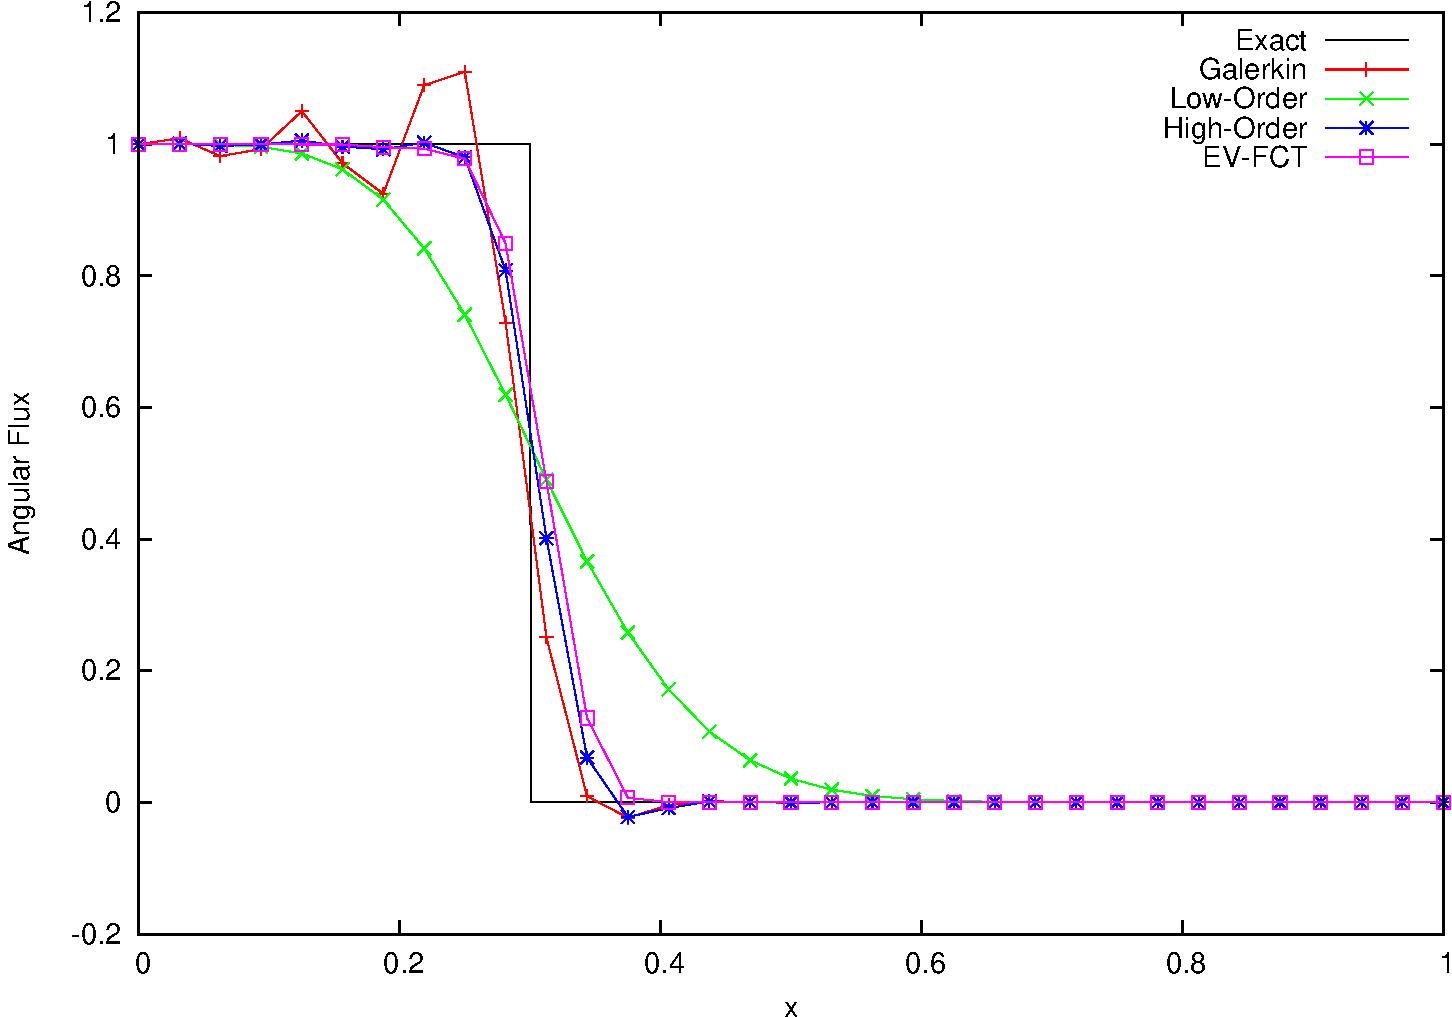
\includegraphics[width=0.20\textwidth]{figures/solutions_3_SSPRK33.pdf}

The given scheme is equally valid for multidimensional problems:
\vspace{\baselineskip}

\begin{minipage}[t]{0.5\linewidth}
  \centering
  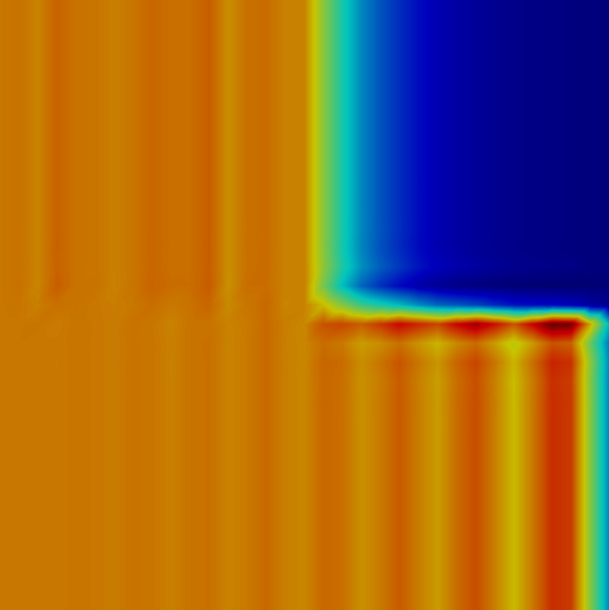
\includegraphics[width=\columnwidth]{figures/Gal2d.png}
  Galerkin
\end{minipage}
\begin{minipage}[t]{0.5\linewidth}
  \centering
  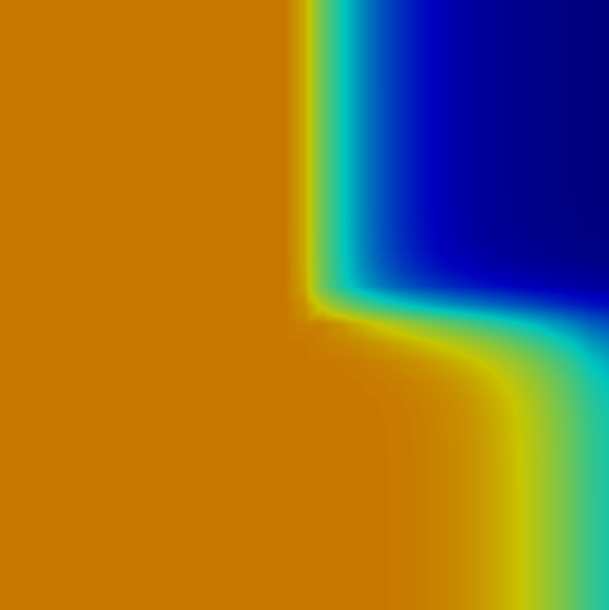
\includegraphics[width=\columnwidth]{figures/GalFCT2d.png}
  FCT
\end{minipage}

\begin{minipage}[t]{0.5\linewidth}
  \centering
  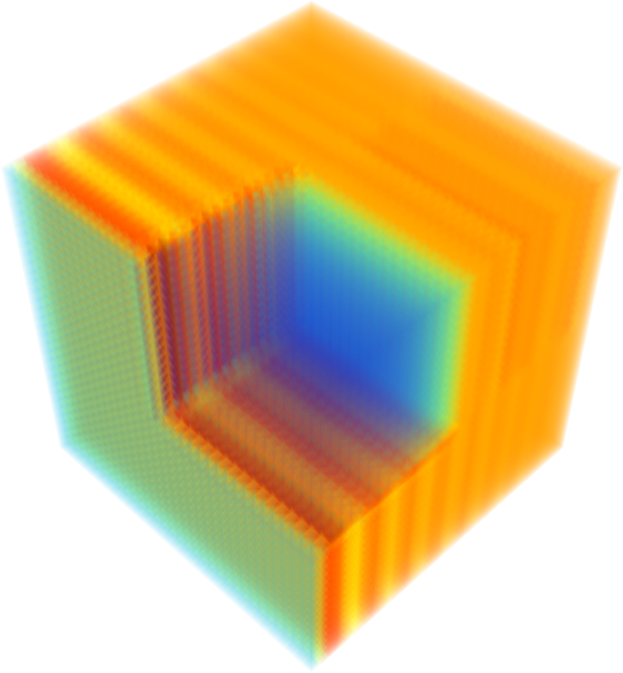
\includegraphics[width=\columnwidth]{figures/Gal_3D.png}
  Galerkin
\end{minipage}
\begin{minipage}[t]{0.5\linewidth}
  \centering
  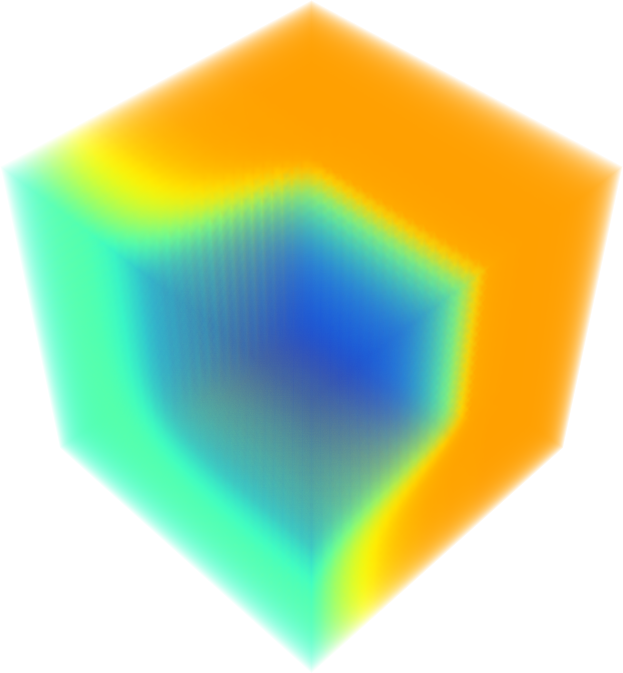
\includegraphics[width=\columnwidth]{figures/GalFCT_3D.png}
  FCT
\end{minipage}

  }

% FOURTH COLUMN
\column{0.25}
  \block{}{
    \setlength{\parskip}{0.5\baselineskip}
    \vspace{-\parskip}
    The figure below shows the convergence results for the void
problem, which because the solution is discontinuous, the theoretical
convergence rates for the high-order scheme are $\frac{3}{4}$ and $\frac{3}{8}$
for L-1 and L-2 error, respectively. The FCT scheme is shown here to
achieve these convergence rates.

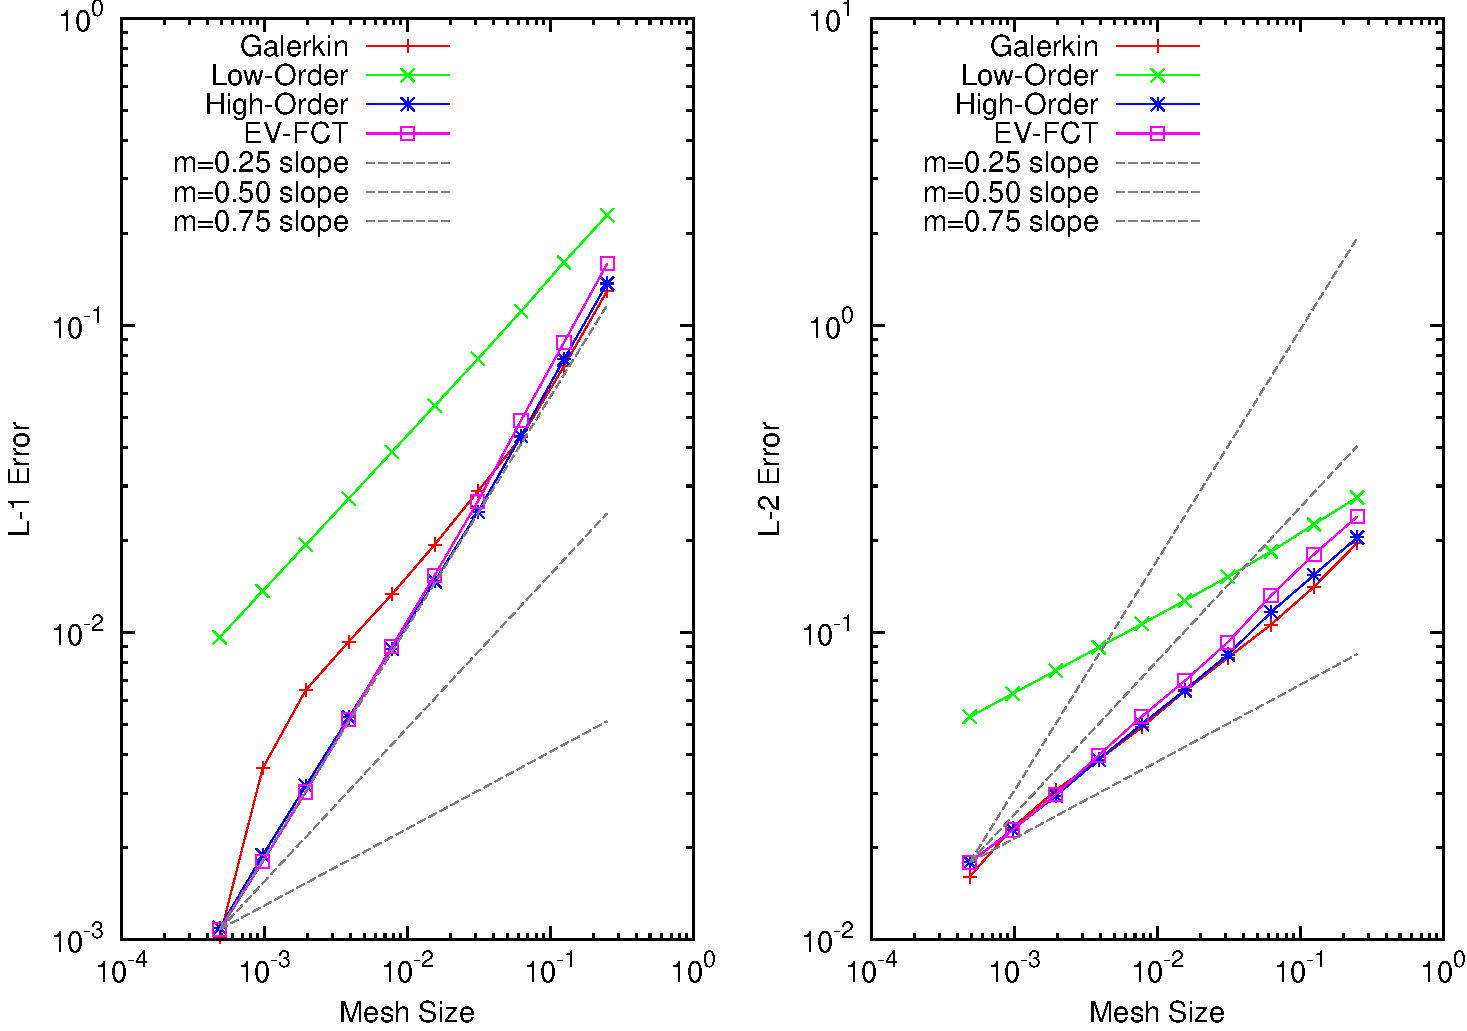
\includegraphics[width=0.20\textwidth]{figures/convergence_3_SSPRK33.pdf}

  }
  \block{\centering CONCLUSIONS}{
    \setlength{\parskip}{0.5\baselineskip}
    \vspace{-\parskip}
    The FCT scheme described in this paper is second-order accurate in space,
converges to the entropy solution, and preserves non-negativity.
Spurious oscillations are mitigated but are not guaranteed to be
eliminated, as smaller magnitude oscillations may exist within the imposed
solution bounds.

% Local solution bounds imposed in the FCT algorithm were derived using the method
% of characteristics and integral transport equation.
% Two sets of solution
% bounds were considered, one considering only values along the upstream
% line segment traversed in a time step, and the other considering a spherical
% neighborhood that encompasses this line segment. The former set of solution
% bounds is much tighter, which has the advantage that there is a smaller range
% of limiting coefficient values that can be used, but has the disadvantage that
% there is less room for antidiffusion.

The traditional FCT phenomenon known as ``stair-stepping'',
``terracing'', or ``plateauing'' is still an open issue, particularly for
fully explicit temporal discretizations; however, these effects
have been shown to diminish or disappear when using SSPRK33 as opposed
to explicit Euler. In addition, these effects are less pronounced for EV-FCT
than in the classic FEM-FCT scheme, which uses the standard Galerkin method as
the high-order method in FCT.

The explicit temporal discretizations of the described FCT scheme yield a
relatively robust algorithm; however, implicit and steady-state discretizations
are much less robust, suffering from severe nonlinear convergence difficulties
in some problems. Implicit schemes become increasingly divergent as the CFL
number is increased. The main complication with implicit and steady-state
FCT schemes is that the imposed solution bounds are implicit with the solution,
and thus the imposed solution bounds change with each iteration of the
nonlinear solver.

  }
  \block{\centering REFERENCES}{
    \begin{center}
      \mbox{}\vspace{-\baselineskip}
      \printbibliography[heading=none]
    \end{center}
  }
  %\block{}{
    %\setlength{\parskip}{\baselineskip}
    %\vspace{-2\parskip}
    %\begin{center}
      %
\includegraphics[width=0.12\textwidth]{figures/neup_logo.jpg}
    %\end{center}
  %}
\end{columns}
\end{document}
